\documentclass{article}

\usepackage{graphicx}
\usepackage{amsmath}
\usepackage{tikz}
\usepackage{pgfkeys}
\usetikzlibrary{calc}

\pgfkeys{
 /compareBlock/.is family, /compareBlock,
 cl/.estore in = \cbCL,
 ch/.estore in = \cbCH,
 ca/.estore in = \cbCA,
 cb/.estore in = \cbCB,
 l/.estore in = \cbL,
 h/.estore in = \cbH,
 a/.estore in = \cbA,
 b/.estore in = \cbB,
 name/.estore in = \cbName,
 default/.style = 
  {ca=black, cb=black, ch=black, cl=black, a=A,b=B, h=H, l=L,name=defaultname}
}

\newcommand{\compareBlock}[2][]{
    \pgfkeys{/compareBlock, default, #1}%
    \coordinate (\cbName_a) at ($(0, 1.33) + #2$);
    \coordinate (\cbName_b) at ($(0, 0.66) + #2$);
    \coordinate (\cbName_l) at ($(1.5, 0.66) + #2$);
    \coordinate (\cbName_h) at ($(1.5, 1.33) + #2$);

    \draw[color=\cbCA] (\cbName_a) -- ++(0.2, 0)node[anchor=west]{\cbA};
    \draw[color=\cbCB] (\cbName_b) -- ++(0.2, 0)node[anchor=west]{\cbB};
    \draw[color=\cbCL] (\cbName_l) -- ++(-0.2, 0)node[anchor=east]{\cbL};
    \draw[color=\cbCH] (\cbName_h) -- ++(-0.2, 0)node[anchor=east]{\cbH};
    \draw[draw=black] #2 rectangle ++(1.5,2);
}
\newcommand{\connectCB}[3]{
    \draw[color=#3] (#1) -- (#2);
}

\begin{document}
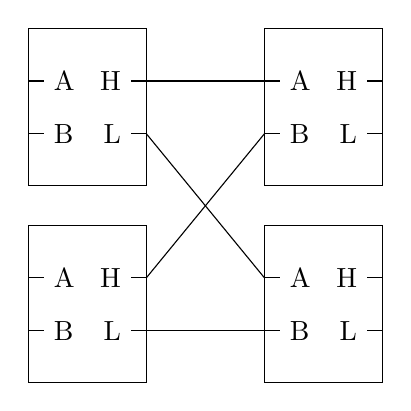
\begin{tikzpicture}
    \compareBlock[name=inL]{(0, 0)}
    \compareBlock[name=inU]{(0, 2.5)}
    \compareBlock[name=outL]{(3, 0)}
    \compareBlock[name=outU]{(3, 2.5)}
    \connectCB{inU_l}{outL_a}{black}
    \connectCB{inL_l}{outL_b}{black}
    \connectCB{inU_h}{outU_a}{black}
    \connectCB{inL_h}{outU_b}{black}
\end{tikzpicture}
\end{document}